\newif\ifalone
\alonefalse
\newif\iftalk
\talkfalse

\ifalone
\documentclass{article}
\usepackage{graphicx}
\usepackage{natbib}
\usepackage{amsfonts}
\usepackage{amssymb}
\usepackage{amsthm}
\usepackage{bm}
\usepackage{Sweave}
\usepackage{lscape}
\usepackage{makeidx}



\title{MCMC}

\author{Jarrod Hadfield (\texttt{j.hadfield@ed.ac.uk})}
\begin{document}
\maketitle
\else
\chapter[Bayesian Statistics \& MCMC]{Bayesian Statistics \& Markov chain Monte Carlo}
\label{chap1}
\fi




There are fundamental differences between classical and Bayesian approaches, but for those of us interested in applied statistics the hope is that these differences do not translate into practical differences, and this is often the case. My advice would be \emph{if} you can fit the same model using different packages and/or methods do so, and if they give very different answers worry. In some cases differences will exist, and it is important to know why, and which method is more appropriate for the data in hand.\\

In the context of a generalised linear mixed model (GLMM), here are what I see as the pro's and cons of using (restricted) maximum likelihood (REML) versus Bayesian Markov chain Monte Carlo (MCMC) Bayesian methods. REML is fast and easy to use, whereas MCMC can be slow and technically more challenging. Particularly challenging is the specification of a sensible prior, something which is a non-issue in a REML analysis. However, analytical results for non-Gaussian GLMM are generally not available, and REML based procedures use approximate likelihood methods that may not work well. MCMC is also an approximation but the accuracy of the approximation increases the longer the analysis is run for, being exact at the limit. In addition REML uses large-sample theory to derive approximate confidence intervals that may have very poor coverage, especially for variance components.  Again, MCMC measures of confidence are exact, up to Monte Carlo error, and provide an easy and intuitive way of obtaining measures of confidence on derived statistics such as ratios of variances, correlations and predictions.\\
 

To illustrate the differences between the approaches lets imagine we've observed several random deviates ({\bf y}) from a standard normal (i.e. $\mu=0$ and $\sigma^{2}=1$).  The likelihood is the probability of the data given the parameters:

\begin{displaymath}
Pr({\bf y} | \mu, \sigma^{2})
\end{displaymath}

This is a conditional distribution, where the conditioning is on the model parameters which are taken as fixed and known. In a way this is quite odd because we've already observed the data, and we don't know what the parameter values are. In a Bayesian analysis we evaluate the conditional probability of the model parameters given the observed data:

\begin{displaymath}
Pr(\mu, \sigma^{2} | {\bf y})
\label{post1-eq}
\end{displaymath}
 
which seems more reasonable, until we realise that this probability is proportional to 

\begin{displaymath}
Pr({\bf y} | \mu, \sigma^{2})Pr(\mu, \sigma^{2})
\end{displaymath}

where the first term is the likelihood, and the second term represents our prior belief in the values that the model parameters could take. Because the choice of prior is rarely justified by an objective quantification of the state of knowledge it has come under criticism, and indeed we will see later that the choice of prior can make a difference. 

\section{Likelihood}

We can generate 5 observations from this distribution using \texttt{rnorm}:

\begin{Schunk}
\begin{Sinput}
> Ndata <- data.frame(y = rnorm(5, mean = 0, sd = sqrt(1)))
> Ndata$y
\end{Sinput}
\begin{Soutput}
[1]  0.01464054  0.87328871 -1.02794620  0.68566463
[5]  0.44943698
\end{Soutput}
\end{Schunk}

We can plot the probability density function for the standard normal using \texttt{dnorm} and we can then place the 5 data on it:

\iftalk
\begin{Schunk}
\begin{Sinput}
> pos.y<-seq(-3,3,0.1)                          # possible values of y
> density<-dnorm(pos.y, mean=0, sd=sqrt(1))     # density of possible values 
> plot(density~pos.y, type="l", ylab="Probability",xlab="", cex.lab=1.5, lwd=2)
> title(xlab="y", col.lab="blue", cex.lab=1.5)
> density.y<-dnorm(Ndata$y, mean=0, sd=sqrt(1)) # density of actual values
> points(density.y~Ndata$y, col="blue", cex=1.75, pch=16)
\end{Sinput}
\end{Schunk}
\else
\begin{Schunk}
\begin{Sinput}
> possible.y<-seq(-3,3,0.1)                          # possible values of y
> Probability<-dnorm(possible.y, mean=0, sd=sqrt(1))     # density of possible values 
> plot(Probability~possible.y, type="l")
> Probability.y<-dnorm(Ndata$y, mean=0, sd=sqrt(1)) # density of actual values
> points(Probability.y~Ndata$y)
\end{Sinput}
\end{Schunk}
\fi

\begin{figure}[!h]
\begin{center}
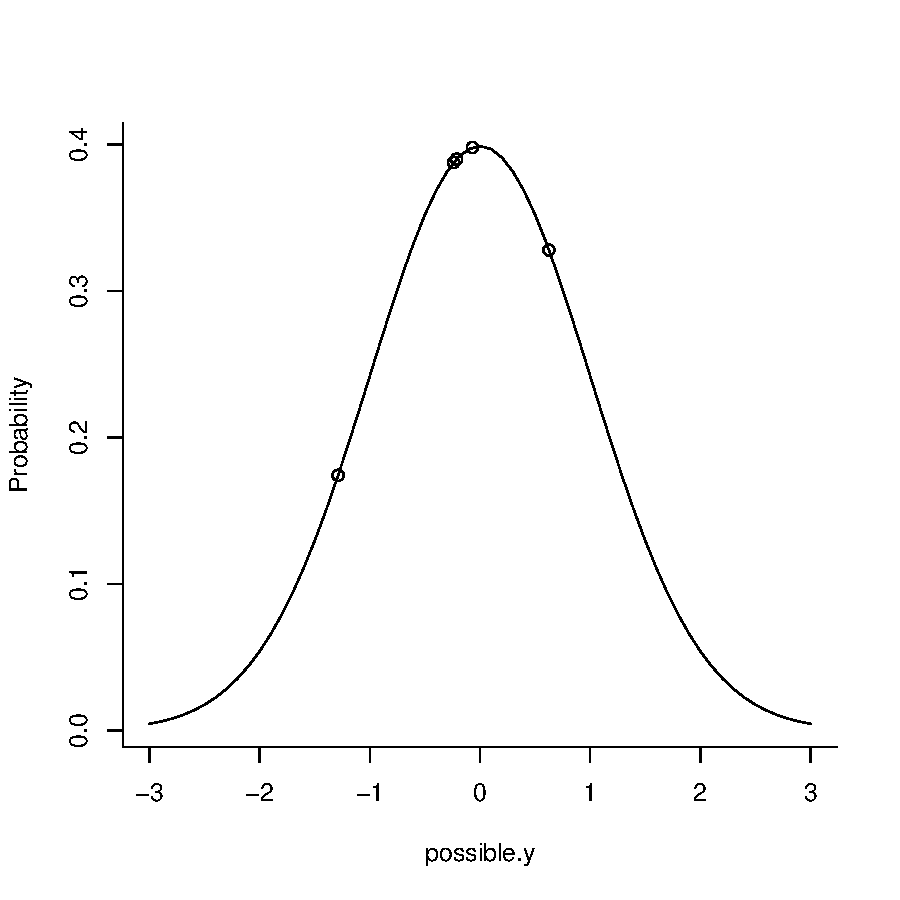
\includegraphics{Lecture1-006}
\end{center}
\caption{Probability density function for the unit normal with the data points overlaid.}
\label{dnorm-fig}
\end{figure}

The likelihood of these data, conditioning on $\mu=0$ and $\sigma^2=1$, is proportional to the product of the densities (read off the y axis on Figure \ref{dnorm-fig}):  

\begin{Schunk}
\begin{Sinput}
> prod(dnorm(Ndata$y, mean = 0, sd = sqrt(1)))
\end{Sinput}
\begin{Soutput}
[1] 0.002907336
\end{Soutput}
\end{Schunk}

Of course we don't know the true mean and variance and so we may want to ask how probable the data would be if, say, $\mu=0$, and $\sigma^2=0.5$:

\iftalk
\else
\fi

\begin{Schunk}
\begin{Sinput}
> prod(dnorm(Ndata$y, mean = 0, sd = sqrt(0.5)))
\end{Sinput}
\begin{Soutput}
[1] 0.004731679
\end{Soutput}
\end{Schunk}

It would seem that the data are more likely under this set of parameters than the true parameters, which we must expect some of the time just from random sampling. To get some idea as to why this might be the case we can overlay the two densities (Figure \ref{dnorm1-fig}), and we can see that although some data points (e.g. 0.873) are more likely with the true parameters, in aggregate the new parameters produce a higher likelihood.\\


\begin{figure}[!h]
\begin{center}
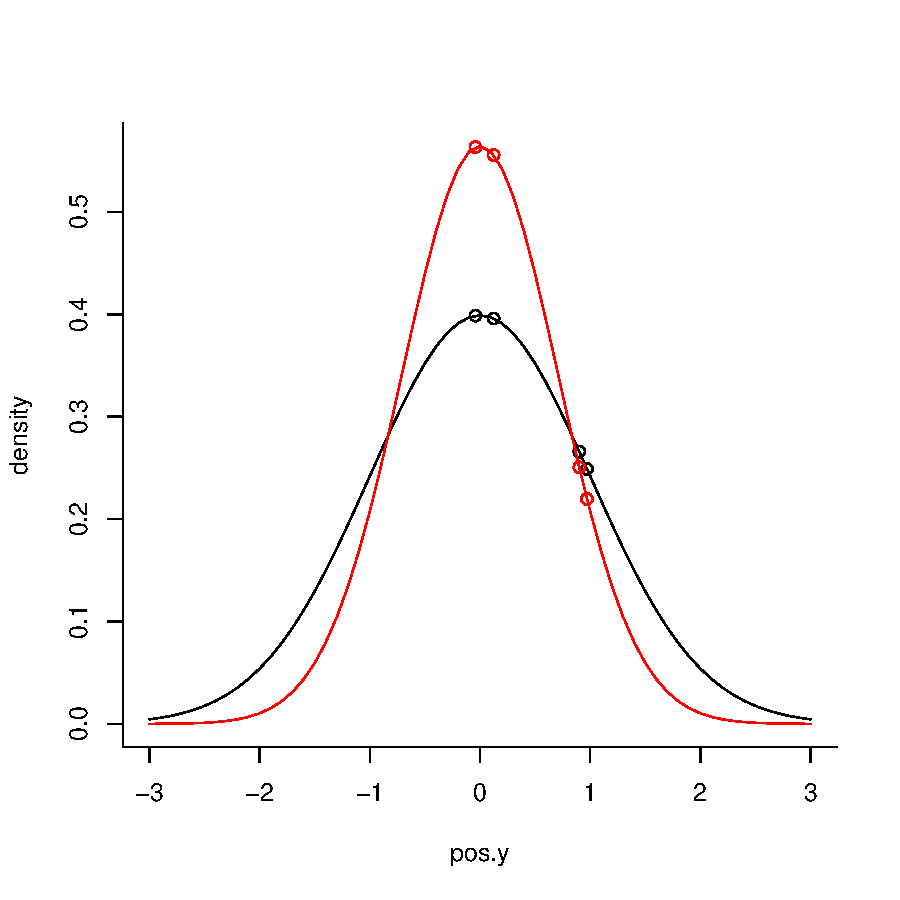
\includegraphics{Lecture1-011}
\end{center}
\caption{Two probability density functions for normal distributions with means of zero, and a variance of one (black line) and a variance of 0.5 (red line).  The data points are overlaid.}
\label{dnorm1-fig}
\end{figure}

The likelihood of the data can be calculated on a grid of possible parameter values to produce a likelihood surface, as in Figure \ref{Lsurface-fig}. The densities on the contours have been scaled so they are relative to the density of the parameter values that have the highest density (the maximum likelihood estimate of the two parameters). Two things are apparent. First, although the surface is symmetric about the line $\mu = \hat{\mu}$ (where $\hat{}$ stands for maximum likelihood estimate) the surface is far from symmetric about the line $\sigma^{2} = \hat{\sigma}^{2}$. Second, there are a large range of parameter values for which the data are only 10 times less likely than if the data were generated under the maximum likelihood estimates.    



\iftalk
\else
\fi

\begin{figure}[!h]
\begin{center}
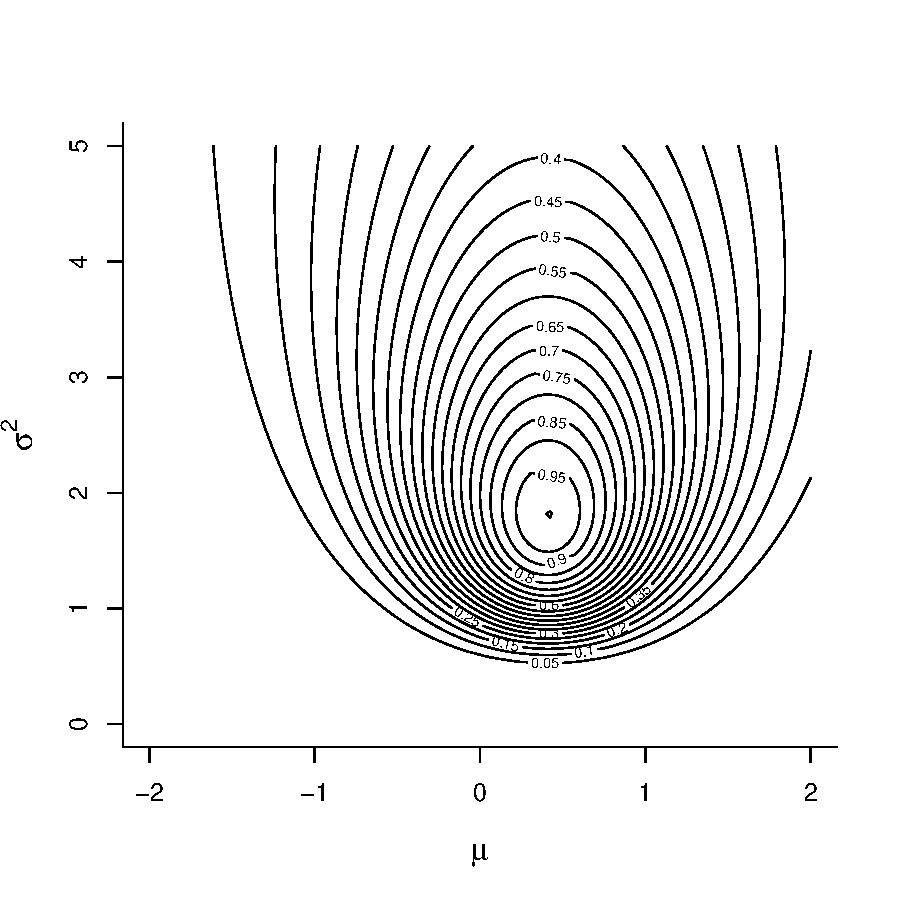
\includegraphics{Lecture1-015}
\end{center}
\caption{Likelihood surface for the likelihood $Pr({\bf y}|\mu, \sigma^{2})$. The likelihood has been normalised so that the maximum likelihood has a value of one.}
\label{Lsurface-fig}
\end{figure}

\subsection{Maximum Likelihood (ML)}

The ML estimator is the combination of $\mu$ and $\sigma^{2}$ that make the data most likely. Although we could evaluate the density on a grid of parameter values (as we did to produce Figure \ref{Lsurface-fig}) in order to locate the maximum, for such a simple problem the ML estimator can be derived analytically. However, so we don't have to meet some nasty maths later, I'll introduce and use one of R's generic optimising routines that can be used to maximise the likelihood function (in practice, the log-likelihood is maximised to avoid numerical problems):


\begin{Schunk}
\begin{Sinput}
> loglik <- function(par, y) {
+     sum(dnorm(y, par[1], sqrt(par[2]), log = TRUE))
+ }
> MLest <- optim(c(mean = 0, var = 1), fn = loglik, 
+     y = Ndata$y, control = list(fnscale = -1, 
+         reltol = 1e-16))$par
\end{Sinput}
\end{Schunk}

\iftalk
\else
\fi

The first call to \texttt{optim} are starting values for the optimisation algorithm, and the second argument (\texttt{fn}) is the function to be maximised. By default \texttt{optim} will try to minimise the function hence multiplying by -1 (\texttt{fnscale = -1}).  The algorithm has successfully found the mode:

\begin{Schunk}
\begin{Sinput}
> MLest
\end{Sinput}
\begin{Soutput}
     mean       var 
0.1990169 0.4587223 
\end{Soutput}
\end{Schunk}

Alternatively we could also fit the model using \texttt{glm}:

\begin{Schunk}
\begin{Sinput}
> m1a.1 <- glm(y ~ 1, data = Ndata)
> summary(m1a.1)
\end{Sinput}
\begin{Soutput}
Call:
glm(formula = y ~ 1, data = Ndata)

Deviance Residuals: 
      1        2        3        4        5  
-0.1844   0.6743  -1.2270   0.4867   0.2504  

Coefficients:
            Estimate Std. Error t value Pr(>|t|)
(Intercept)   0.1990     0.3386   0.588    0.588

(Dispersion parameter for gaussian family taken to be 0.5734029)

    Null deviance: 2.2936  on 4  degrees of freedom
Residual deviance: 2.2936  on 4  degrees of freedom
AIC: 14.293

Number of Fisher Scoring iterations: 2
\end{Soutput}
\end{Schunk}
 
Here we see that although the estimate of the mean (intercept) is the same, the estimate of the variance (the dispersion parameter: 0.573) is higher when fitting the model using \texttt{glm}. In fact the ML estimate is a factor of $\frac{n}{n-1}$ smaller.

\begin{Schunk}
\begin{Sinput}
> MLest["var"] * (5/4)
\end{Sinput}
\begin{Soutput}
      var 
0.5734029 
\end{Soutput}
\end{Schunk}

\subsection{Restricted Maximum Likelihood (REML)}

To see why this happens, imagine if we had only observed the first two values of $y$ (Figure \ref{muvar-fig}). The variance is defined as the average squared distance between a random variable and the \emph{true} mean. However, the ML estimator of the variance is the average squared distance between a random variable and the ML \emph{estimate} of the mean. Since the ML estimator of the mean is the average of the two numbers (the dashed line) then the average squared distance will always be smaller than if the true mean was used, unless the ML estimate of the mean and the true mean coincide. This is why we divide by $n-1$ when estimating the variance from the sum of squares, and is the motivation behind REML.

\iftalk
\else
\fi

\begin{figure}[!h]
\begin{center}
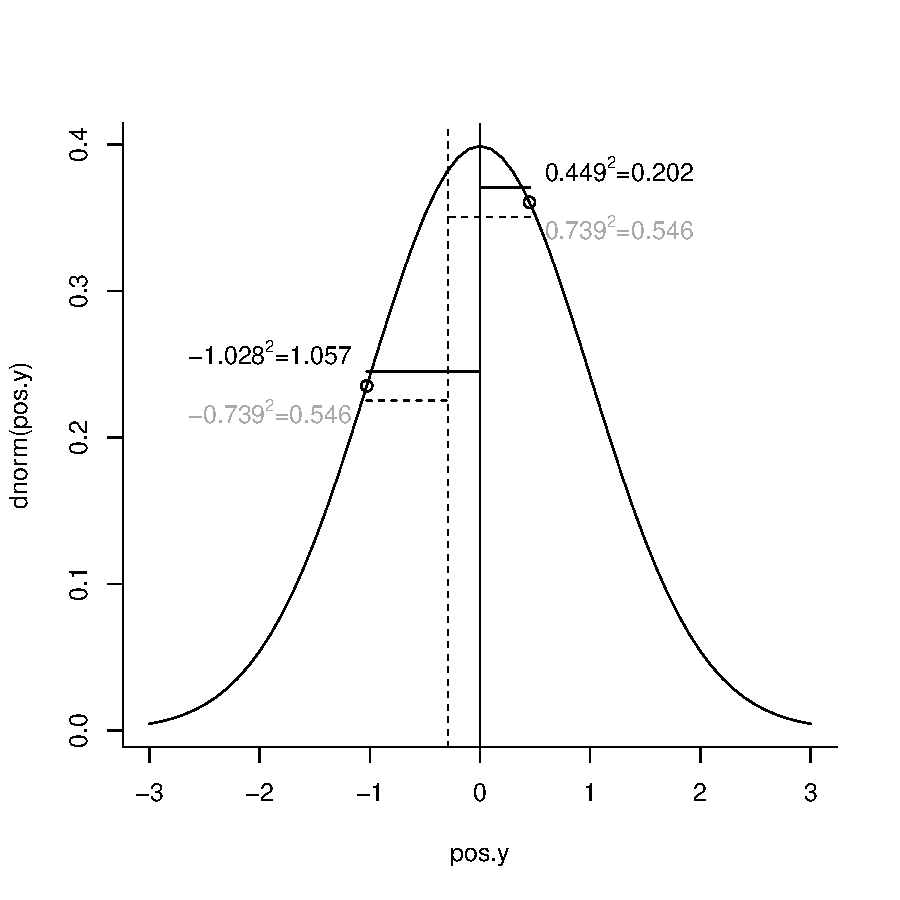
\includegraphics{Lecture1-023}
\end{center}
\caption{Probability density function for the unit normal with 2 realisations overlaid. The solid vertical line is the true mean, whereas the vertical dashed line is the mean of the two realisations (the ML estimator of the mean). The variance is the expected squared distance between the true mean and the realisations. The ML estimator of the variance is the average squared distance between the ML mean and the realisations (horizontal dashed lines), which is always smaller than the average squared distance between the true mean and the realisations (horizontal solid lines)}
\label{muvar-fig}
\end{figure}

\newpage
\section{Prior Distribution}

\texttt{MCMCglmm} uses an inverse Wishart prior for the (co)variances and a normal prior for the fixed effects. In versions $>1.13$ parameter expanded models can be used which enable prior specifications from the the scaled non-central F-distribution \citep{Gelman.2006}. Here, we will focus on specifying a prior for a single fixed effect ($\mu$) and a single variance component using the inverse-Wishart to highlight some of the issues. I strongly recommend reading the section \ref{secPX-p} on parameter expanded priors as these can be less informative than the inverse-Wishart under many situations.\\

For a single variance component the inverse Wishart takes two scalar parameters, \texttt{V} and \texttt{nu}. The distribution tends to a point mass on \texttt{V} as the degree of belief parameter, \texttt{nu} goes to infinity. The distribution tends to be right skewed when \texttt{nu} is not very large, with a mode of $\frac{\texttt{V}^{\ast}\texttt{nu}}{\texttt{nu}+2}$ but a mean of $\frac{\texttt{V}^{\ast}\texttt{nu}}{\texttt{nu}-2}$ (which is not defined for $\texttt{nu}<2$).\footnote{The inverse gamma is a special case of the inverse Wishart, although it is parametrised using \texttt{shape} and \texttt{scale}, where $\texttt{nu}=2\ast\texttt{shape}$ and $\texttt{V} = \frac{\texttt{scale}}{\texttt{shape}}$ (or $\texttt{shape} = \frac{\texttt{nu}}{2}$ and $\texttt{scale} = \frac{\texttt{nu}*\texttt{V}}{2}$). \texttt{MCMCpack} provides a density function (\texttt{dinvgamma}) for the inverse gamma distribution.}\\

As before, we can evaluate and plot density functions in order to visualise what the distribution looks like. Figure \ref{dinvgamma-fig} plots the probability density functions holding \texttt{V} equal to one but with \texttt{nu} varying.\\

\iftalk
\else
\fi

\iftalk
\else
\fi

\begin{figure}[!h]
\begin{center}
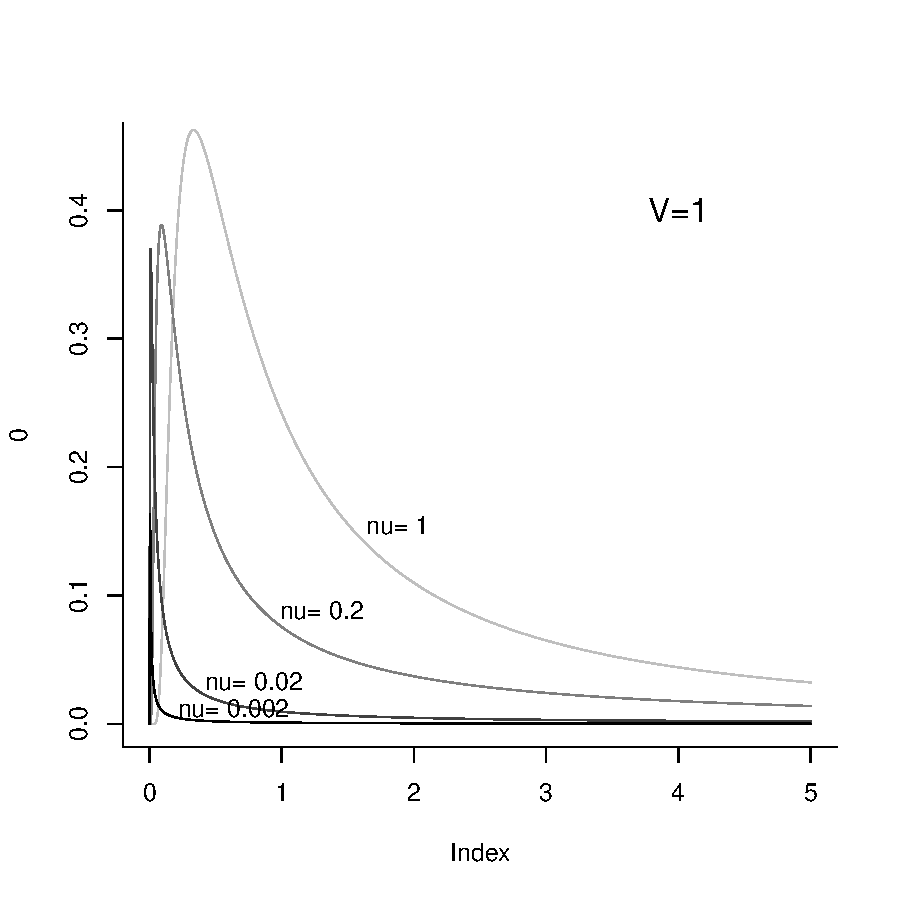
\includegraphics{Lecture1-027}
\end{center}
\caption{Probability density function for a univariate inverse Wishart with the variance at the limit set to 1 (\texttt{V=1}) and varying degree of belief parameter (\texttt{nu}). With \texttt{V=1} these distributions are equivalent to inverse gamma distributions with shape and scale parameters set to \texttt{nu}/2.}
\label{dinvgamma-fig}
\end{figure}

A probability distribution must integrate to one because a variable must have some value. It therefore seems reasonable that when specifying a prior, care must be taken that this condition is met. In the example here where \texttt{V} is a single variance this condition is met if \texttt{V>0} and \texttt{nu>0}.  If this condition is not met then the prior is said to be improper, and in WinBUGS (and possibly other software) improper priors cannot be specified.  Although great care has to be taken when using improper priors, \texttt{MCMCglmm} does allow them as they have some useful properties, and some common improper priors are discussed in section \ref{IP-sec}. However, for now we will use the prior specification \texttt{V=1} and \texttt{nu=0.002} which is frequently used for variance components. For the mean we will use a diffuse normal prior centred around zero but with very large variance ($10^{8}$). If the variance is finite then the prior is always proper.\\

As before we can write a function for calculating the (log) prior probability:

\begin{Schunk}
\begin{Sinput}
> logprior <- function(par, priorR, priorB) {
+     dnorm(par[1], mean = priorB$mu, sd = sqrt(priorB$V), 
+         log = TRUE) + log(dinvgamma(par[2], shape = priorR$nu/2, 
+         scale = (priorR$nu * priorR$V)/2))
+ }
\end{Sinput}
\end{Schunk}

where \texttt{priorR} is a list with elements \texttt{V} and \texttt{nu} specifying the prior for the variance, and \texttt{priorB} is a list with elements \texttt{mu} and \texttt{V} specifying the prior for the mean. \texttt{MCMCglmm} takes these prior specifications as a list: 

\begin{Schunk}
\begin{Sinput}
> prior <- list(R = list(V = 1, nu = 0.002), B = list(mu = 0, 
+     V = 1e+08))
\end{Sinput}
\end{Schunk}


\section{Posterior Distribution}

  To obtain a posterior density we need to multiply the likelihood by the prior probability for that set of parameters. We can write a function for doing this: 

\begin{Schunk}
\begin{Sinput}
> loglikprior <- function(par, y, priorR, priorB) {
+     loglik(par, y) + logprior(par, priorR, priorB)
+ }
\end{Sinput}
\end{Schunk}

and we can overlay the posterior densities on the likelihood surface we calculated before (Figure \ref{Lsurface-fig}).\\


\iftalk
\else
\fi

\begin{figure}[!h]
\begin{center}
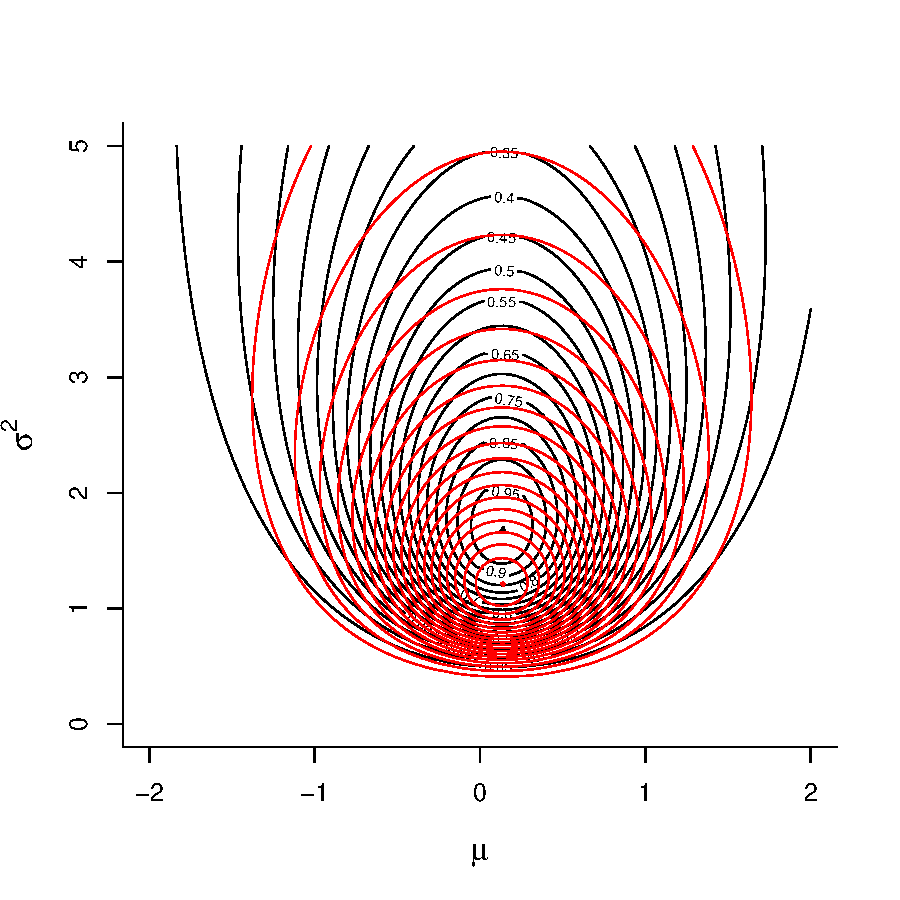
\includegraphics{Lecture1-034}
\end{center}
\caption{Likelihood surface for the likelihood $Pr({\bf y}|\mu, \sigma^{2})$ in black, and the posterior distribution $Pr(\mu, \sigma^{2} | {\bf y})$ in red.  The likelihood has been normalised so that the maximum likelihood has a value of one, and the posterior distribution has been normalised so that the posterior mode has a value of one. The prior distributions  $Pr(\mu)\sim N(0, 10^8)$ and  $Pr(\sigma^{2})\sim IW(\texttt{V}=1, \texttt{nu}=0.002)$ were used.}
\label{Psurface-fig}
\end{figure}


The prior has some influence on the posterior mode of the variance, and we can use an optimisation algorithm again to locate the mode:  

\begin{Schunk}
\begin{Sinput}
> Best <- optim(c(mean = 0, var = 1), fn = loglikprior, 
+     y = Ndata$y, priorR = prior$R, priorB = prior$B, 
+     control = list(fnscale = -1, reltol = 1e-16))$par
> Best
\end{Sinput}
\begin{Soutput}
     mean       var 
0.1990169 0.3278509 
\end{Soutput}
\end{Schunk}

\iftalk
\else
\fi

The posterior mode for the mean is identical to the ML estimate, but the posterior mode for the variance is even less than the ML estimate which is known to be downwardly biased. The reason that the ML estimate is downwardly biased is because it did no take into account the uncertainty in the mean. In a Bayesian analysis we can do this by evaluating the marginal distribution of $\sigma^{2}$ and averaging over the uncertainty in the mean.

\subsection{Marginal Posterior Distribution}

The marginal distribution is often of primary interest in statistical inference, because it represents our knowledge about a parameter given the data: 

\begin{displaymath}
Pr(\sigma^{2} | {\bf y}) \propto \int Pr(\mu, \sigma^{2} | {\bf y})d\mu
\label{marg-eq}
\end{displaymath}

after averaging over any nuisance parameters, such as the mean in this case.\\  

Obtaining the marginal distribution analytically is usually impossible, and this is where MCMC approaches prove useful.  We can fit this model in \texttt{MCMCglmm} pretty much in the same way as we did using \texttt{glm}:


\begin{Schunk}
\begin{Sinput}
> m1a.2 <- MCMCglmm(y ~ 1, data = Ndata, prior = prior, 
+     thin = 1, verbose = FALSE)
\end{Sinput}
\end{Schunk}

The Markov chain is drawing random (but often correlated) samples from the joint posterior distribution (depicted by the red contours in Figure \ref{Psurface-fig}).  The element of the output called \texttt{Sol} contains the distribution for the mean, and the element called \texttt{VCV} contains the distribution for the variance. We can produce a scatter plot:

\begin{Schunk}
\begin{Sinput}
> points(cbind(m1a.2$Sol, m1a.2$VCV))
\end{Sinput}
\end{Schunk}

and we see that MCMCglmm is sampling the same distribution as the posterior distribution calculated on a grid of possible parameter values (Figure \ref{PsurfaceMCMC-fig}).\\

\iftalk
\else
\fi

\begin{figure}[!h]
\begin{center}
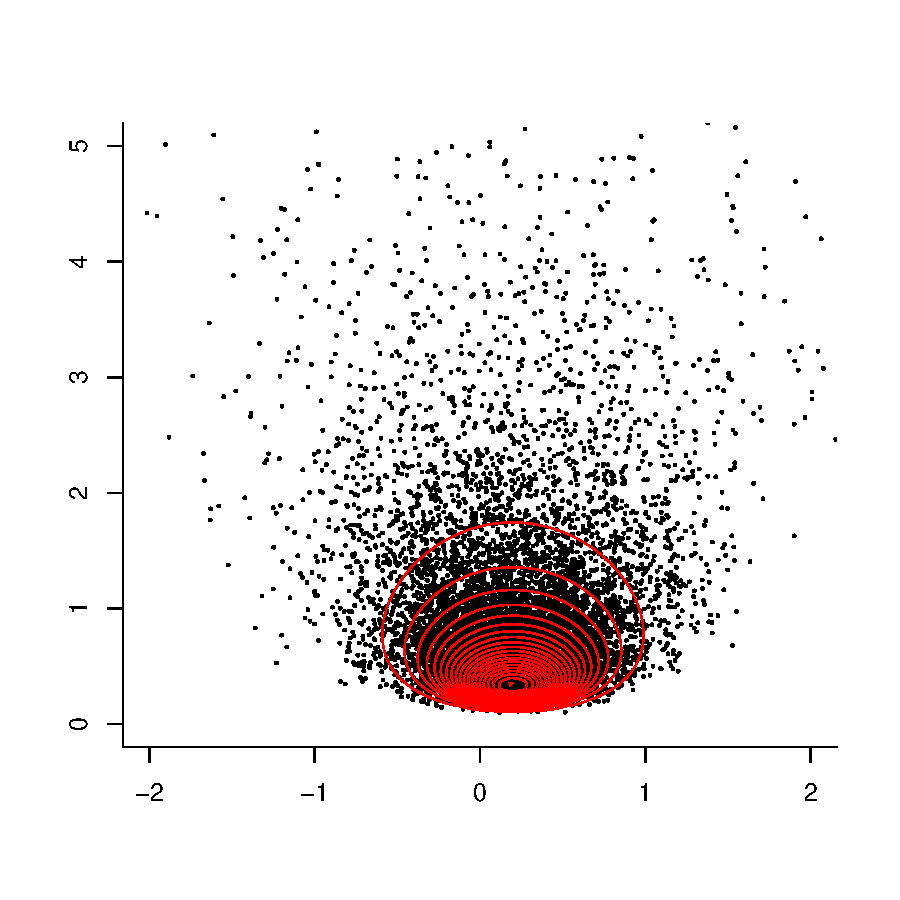
\includegraphics{Lecture1-041}
\end{center}
\caption{The posterior distribution $Pr(\mu, \sigma^{2} | {\bf y})$. The black dots are samples from the posterior using MCMC, and the red contours are calculated by evaluating the posterior density on a grid of parameter values. The contours are normalised so that the posterior mode has a value of one.}
\label{PsurfaceMCMC-fig}
\end{figure}

A very nice property of MCMC is that we can normalise the density so that it integrates to 1 (a true probability) rather than normalising it with respect to some other aspect of the distribution, such as the density at the ML estimator or the joint posterior mode as in Figures \ref{Lsurface-fig} and \ref{Psurface-fig}. To make this clearer, imagine we wanted to know how much more probable the unit normal (i.e. with $\mu=0$ and $\sigma^{2}=1$) was than a normal distribution with the posterior modal parameters. We can calculate this by taking the ratio of the posterior densities at these two points:  \\ 
 

\begin{Schunk}
\begin{Sinput}
> exp(loglikprior(Best, Ndata$y, prior$R, prior$B) - 
+     loglikprior(c(0, 1), Ndata$y, prior$R, prior$B))
\end{Sinput}
\begin{Soutput}
[1] 5.207646
\end{Soutput}
\end{Schunk}


Now, if we wanted to know the probability that the parameters lay in the region of parameter space we were plotting, i.e. lay in the square $\mu = (-2,2)$ and $\sigma^{2} = (0,5)$ then this would be more difficult. We would have to evaluate the density at a much larger range of parameter values than we had done, ensuring that we had covered all regions with positive probability. Because MCMC has sampled the distribution randomly, this probability will be equal to the expected probability that we have drawn an MCMC sample from the region. We can obtain an estimate of this by seeing what proportion of our actual samples lie in this square:

\begin{Schunk}
\begin{Sinput}
> prop.table(table(m1a.2$Sol > -2 & m1a.2$Sol < 
+     2 & m1a.2$VCV < 5))
\end{Sinput}
\begin{Soutput}
 FALSE   TRUE 
0.0239 0.9761 
\end{Soutput}
\end{Schunk}

There is Monte Carlo error in the answer (0.976) but if we collect a large number of samples then this can be minimised.\\ 

Using a similar logic we can obtain the marginal distribution of the variance by simply evaluating the draws in \texttt{VCV} ignoring (averaging over) the draws in \texttt{Sol}:

\iftalk
\else
\begin{Schunk}
\begin{Sinput}
> hist(m1a.2$VCV[which(m1a.2$VCV < 5)])
> abline(v = Best["var"], col = "red")
\end{Sinput}
\end{Schunk}
\fi

\begin{figure}[!h]
\begin{center}
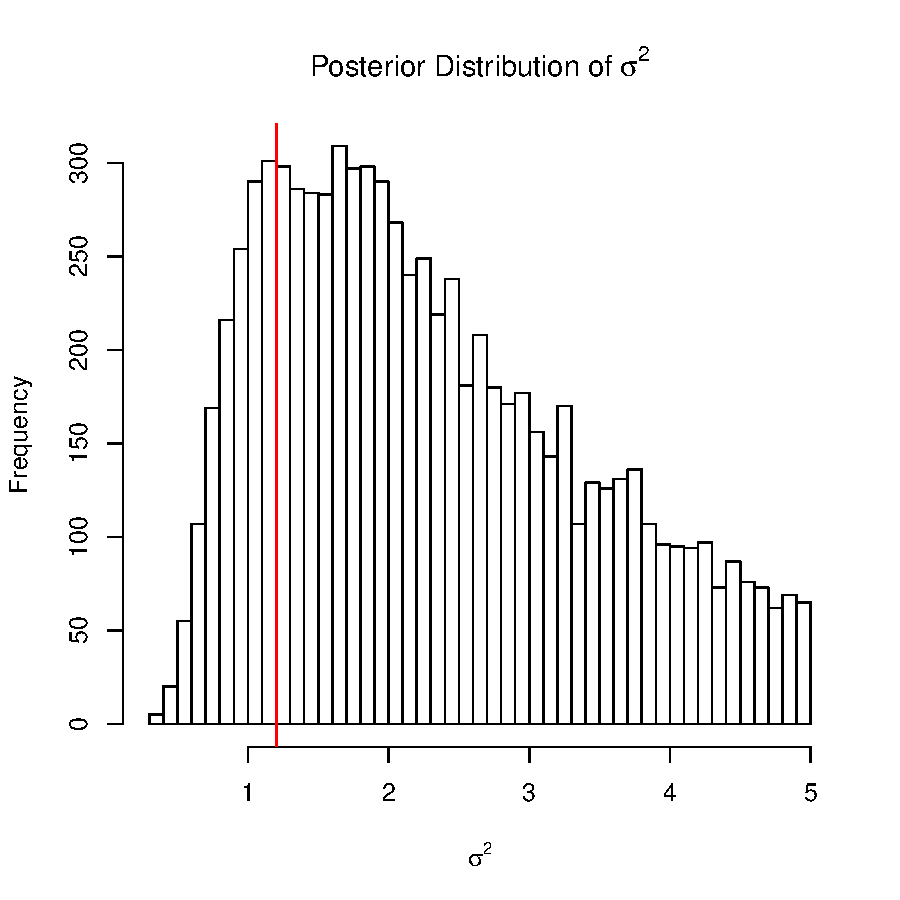
\includegraphics{Lecture1-049}
\end{center}
\caption{Histogram of samples from the marginal distribution of the variance $Pr(\sigma^{2} | {\bf y})$ using MCMC. The vertical line is the joint posterior mode, which differs slightly from the marginal posterior mode (the peak of the marginal distribution).}
\label{PsurfaceMCMC-fig}
\end{figure}

In this example (see Figure \ref{PsurfaceMCMC-fig}) the marginal mode and the joint mode are very similar, although this is not necessarily the case and can depend both on the data and the prior. Section \ref{IP-sec} introduces improper priors that are non-informative with regard to the marginal distribution of a variance.\\

\section{MCMC}

In order to be confident that \texttt{MCMCglmm} has successfully sampled the posterior distribution it will be necessary to have a basic understanding of MCMC methods. MCMC methods are often used when the joint posterior distribution cannot be derived analytically, which is nearly always the case. MCMC relies on the fact that although we cannot derive the complete posterior, we can calculate the height of the posterior distribution at a particular set of parameter values, as we did to obtain the contour plot in Figure \ref{Psurface-fig}. However, rather than going systematically through every likely combination of $\mu$ and $\sigma$ and calculate the height of the distribution at regular distances, MCMC moves stochastically through parameter space, hence the name `Monte Carlo'.\\   

\subsection{Starting values}

First we need to initialise the chain and specify a set of parameter values from which the chain can start moving through parameter space. Ideally we would like to pick a region of high probability, as we do not want to waste time wandering through regions of low probability: we are not so interested in determining the height of the distribution far outside of  Figure \ref{Psurface-fig} as it is virtually flat and close to zero (or at least we hope so!).  Although starting configurations can be set by the user using the \texttt{start} argument, in general the heuristic techniques used by \texttt{MCMCglmm} seem to work quite well. We will denote the parameter values of the starting configuration (time $t=0$) as $\mu_{t=0}$ and ${\sigma^{2}}_{t=0}$. There are several ways in which we can get the chain to move in parameter space, and \texttt{MCMCglmm} uses a combination of Gibbs sampling, slice sampling and Metropolis-Hastings updates. To illustrate, it will be easier to turn the contour plot of the posterior distribution into a perspective plot (Figure \ref{Psurface.persp-fig}).

  

\begin{figure}[!h]
\begin{center}
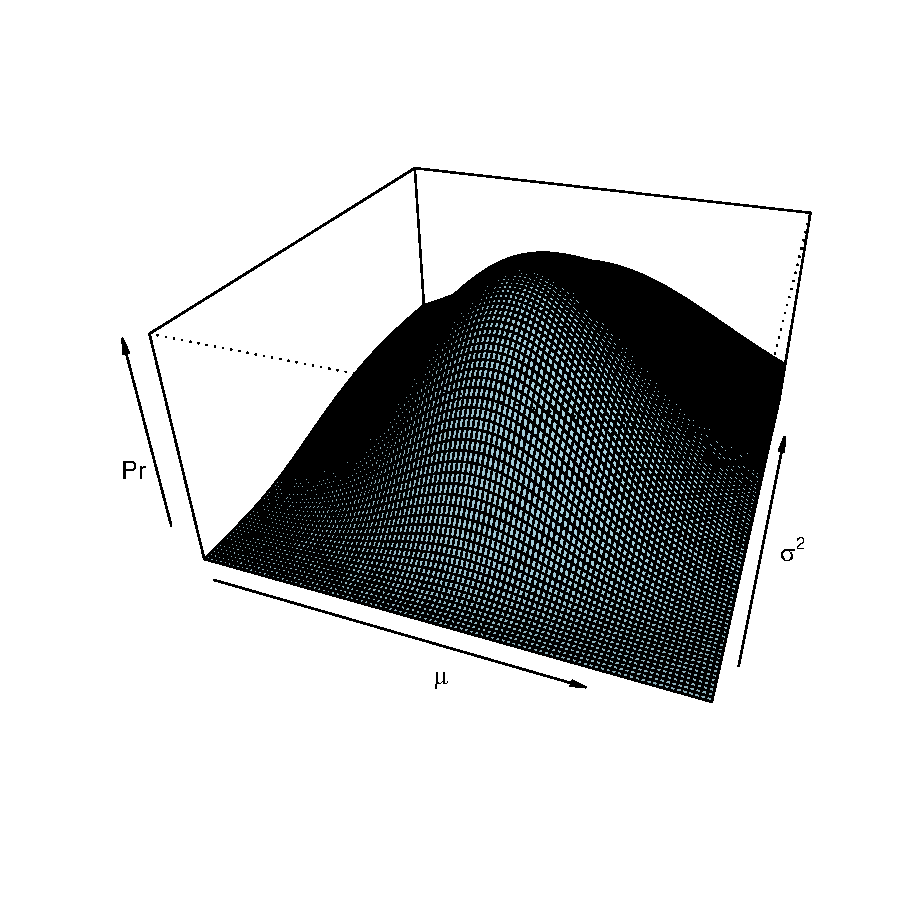
\includegraphics{Lecture1-052}
\end{center}
\caption{The posterior distribution $Pr(\mu, \sigma^{2} | {\bf y})$. This perspective plot is equivalent to the contour plot in Figure \ref{Psurface-fig}}
\label{Psurface.persp-fig}
\end{figure}


\subsection{Metrpolis-Hastings updates}

After initialising the chain we need to decide where to go next, and this decision is based on two rules.  First we have to generate a candidate destination, and then we need to decide whether to go there or stay where we are.  There are many ways in which we could generate candidate parameter values, and \texttt{MCMCglmm} uses a well tested and simple method. A random set of coordinates are picked from a multivariate normal distribution that is entered on the initial coordinates  $\mu_{t=0}$ and $\sigma^{2}_{t=0}$.  We will denote this new set of parameter values as  $\mu_{new}$ and $\sigma^{2}_{new}$. The question then remains whether to move to this new set of parameter values or remain at our current parameter values now designated as old $\mu_{old}=\mu_{t=0}$ and $\sigma^{2}_{old}=\sigma^{2}_{t=0}$.  If the posterior probability for the new set of parameter values is greater, then the chain moves to this new set of parameters and the chain has successfully completed an iteration: ($\mu_{t=1} = \mu_{new}$ and $\sigma^{2}_{t=1}=\sigma^{2}_{new}$).  If the new set of parameter values has a lower posterior probability then the chain may move there, but not all the time.  The probability that the chain moves to low lying areas, is determined by the relative difference between the old and new posterior probabilities.  If the posterior probability for $\mu_{new}$ and $\sigma^{2}_{new}$ is 5 times less than the posterior probability for $\mu_{old}$ and $\sigma^{2}_{old}$, then the chain would move to the new set of parameter values 1 in 5 times. If the move is successful then we set $\mu_{t=1} = \mu_{new}$ and $\sigma^{2}_{t=1}=\sigma^{2}_{new}$ as before, and if the move is unsuccessful then the chain stays where it is ($\mu_{t=1} = \mu_{old}$ and $\sigma^{2}_{t=1}=\sigma^{2}_{old}$).  Using these rules we can record where the chain has travelled and generate an approximation of the posterior distribution.  Basically, a histogram of Figure \ref{Psurface.persp-fig}.\\
 
\subsection{Gibbs Sampling}

Gibbs sampling is a special case of Metropolis-Hastings updating, and \texttt{MCMCglmm} uses Gibbs sampling to update most parameters.  In the Metropolis-Hastings example above, the Markov Chain was allowed to move in both directions of parameter space simultaneously.  An equally valid approach would have been to set up two Metropolis-Hastings schemes where the chain was first allowed to move along the $\mu$ axis, and then along the $\sigma^{2}$ axis. In Figure \ref{Psurface.persp2-fig} I have cut the posterior distribution of Figure \ref{Psurface.persp-fig} in half, and the edge of the surface facing left is the conditional distribution of $\mu$ given that $\sigma^{2}=1$:


\begin{equation}
Pr(\mu |\sigma^{2}=1, \bm{y}).
\end{equation}




\begin{figure}[!h]
\begin{center}
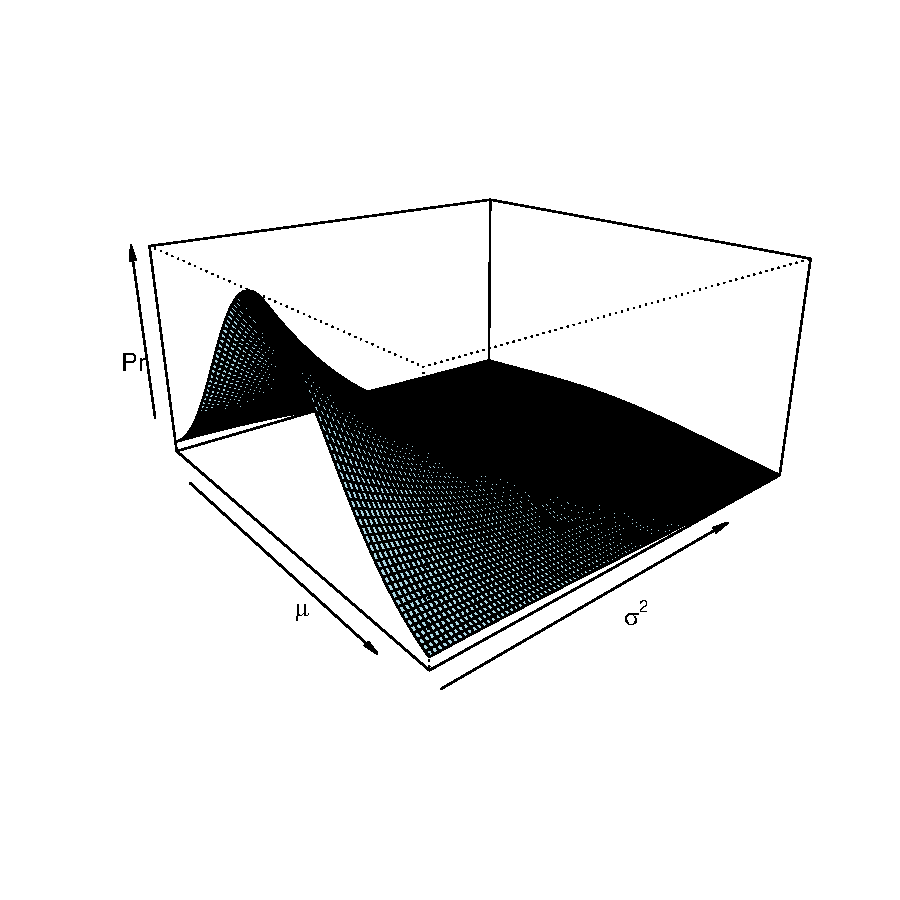
\includegraphics{Lecture1-055}
\end{center}
\caption{The posterior distribution $Pr(\mu, \sigma^{2} | {\bf y})$, but only for values of $\sigma^{2}$ between 1 and 5, rather than 0 to 5 (Figure \ref{Psurface.persp-fig}). The 
edge of the surface facing left is the conditional distribution of the mean when $\sigma^{2}=1$ ($Pr(\mu | {\bf y}, \sigma^{2}=1)$). This conditional distribution follows a normal distribution.}
\label{Psurface.persp2-fig}
\end{figure}

 In some cases, the equation that describes this conditional distribution can be derived despite the equation for the complete joint distribution of Figure \ref{Psurface.persp-fig} remaining unknown.  When the conditional distribution of $\mu$ is known we can use Gibbs sampling. Lets say the chain at a particular iteration is located at $\sigma^{2}=1$.  If we updated $\mu$ using a Metropolis-Hastings algorithm we would generate a candidate value and evaluate its relative probability compared to the old value.  This procedure would take place in the slice of posterior facing left in Figure \ref{Psurface.persp2-fig}. However, because we know the actual equation for this slice we can just generate a new value of $\mu$ directly. This is Gibbs sampling.  The slice of the posterior that we can see in Figure \ref{Psurface.persp2-fig} actually has a normal distribution. Because of the weak prior this normal distribution has a mean close to the mean of $\bf{y}$ and a variance close to $\frac{\sigma^{2}}{n} = \frac{1}{n}$.  Gibbs sampling can be much more efficient than Metropolis-Hastings updates, especially when high dimensional conditional distributions are known, as is typical in GLMMs. A technical description of the sampling schemes used by \texttt{MCMCglmm} is given in appendix \ref{MCMC-app}, but is perhaps not important to know.

\subsection{Slice Sampling}

If the distribution can be factored such that one factor is a distribution from which truncated random variables can be drawn, then the slice sampling methods of \citet{Damien.1999} can be used. The latent variables in univariate binary models can be updated in this way if \texttt{slice=TRUE} is specified in the call to \texttt{MCMCglmm}. In these models, slice sampling is only marginally more efficient than adaptive Metropolis-Hastings updates when the residual variance is fixed. However, for parameter expanded binary models where the residual variance is not fixed, the slice sampler can be much more efficient.

\subsection{MCMC Diagnostics}

When fitting a model using \texttt{MCMCglmm} the parameter values through which the Markov chain has travelled are stored and returned.  The length of the chain (the number of iterations) can be specified using the \texttt{nitt} argument\footnote{The double \texttt{t} is because I cannot spell.} (the default is 13,000), and should be long enough so that the posterior approximation is valid.  If we had known the joint posterior distribution in Figure \ref{Psurface.persp-fig} we could have set up a Markov chain that sampled directly from the posterior.  If this had been the case, each successive value in the Markov chain would be independent of the previous value after conditioning on the data, ${\bf y}$, and a thousand iterations of the chain would have produced a histogram that resembled Figure \ref{Psurface.persp-fig} very closely.  However, generally we do not know the joint posterior distribution of the parameters, and for this reason the parameter values of the Markov chain at successive iterations are usually not independent and care needs to be taken regarding the validity of the approximation.  \texttt{MCMCglmm} returns the Markov chain as \texttt{mcmc} objects, which can be analysed using the \texttt{coda} package.  The function \texttt{autocorr} estimates the level of non-independence between successive samples in the chain:

\begin{Schunk}
\begin{Sinput}
> autocorr(m1a.2$Sol)
\end{Sinput}
\begin{Soutput}
, , (Intercept)

        (Intercept)
Lag 0   1.000000000
Lag 1   0.023715850
Lag 5   0.007823033
Lag 10 -0.011490974
Lag 50  0.008903345
\end{Soutput}
\begin{Sinput}
> autocorr(m1a.2$VCV)
\end{Sinput}
\begin{Soutput}
, , units

              units
Lag 0   1.000000000
Lag 1   0.228517764
Lag 5  -0.007597471
Lag 10 -0.004843682
Lag 50  0.006178729
\end{Soutput}
\end{Schunk}

 The correlation between successive samples is low for the mean (0.024) but a bit high for the variance (0.229).  When auto-correlation is high the chain needs to be run for longer, and this can lead to storage problems for high dimensional problems. The argument \texttt{thin} can be passed to \texttt{MCMCglmm} specifying the intervals at which the Markov chain is stored. In model \texttt{m1a.2} we specified \texttt{thin=1} meaning we stored every iteration (the default is \texttt{thin=10}). I usually aim to store 1,000-2,000 iterations and have the autocorrelation between successive \emph{stored} iterations less than 0.1.\\

The approximation obtained from the Markov chain is conditional on the set of parameter values that were used to initialise the chain.  In many cases the first iterations show a strong dependence on the starting parametrisation, but as the chain progresses this dependence may be lost.  As the dependence on the starting parametrisation diminishes the chain is said to converge and the argument \texttt{burnin} can be passed to \texttt{MCMCped} specifying the number of iterations which must pass before samples are stored. The default burn-in period is 3,000 iterations. Assessing convergence of the chain is notoriously difficult, but visual inspection and diagnostic tools such as \texttt{gelman.diag} often suffice.

\begin{Schunk}
\begin{Sinput}
> plot(m1a.2$Sol)
\end{Sinput}
\end{Schunk}

\begin{figure}[!h]
\begin{center}
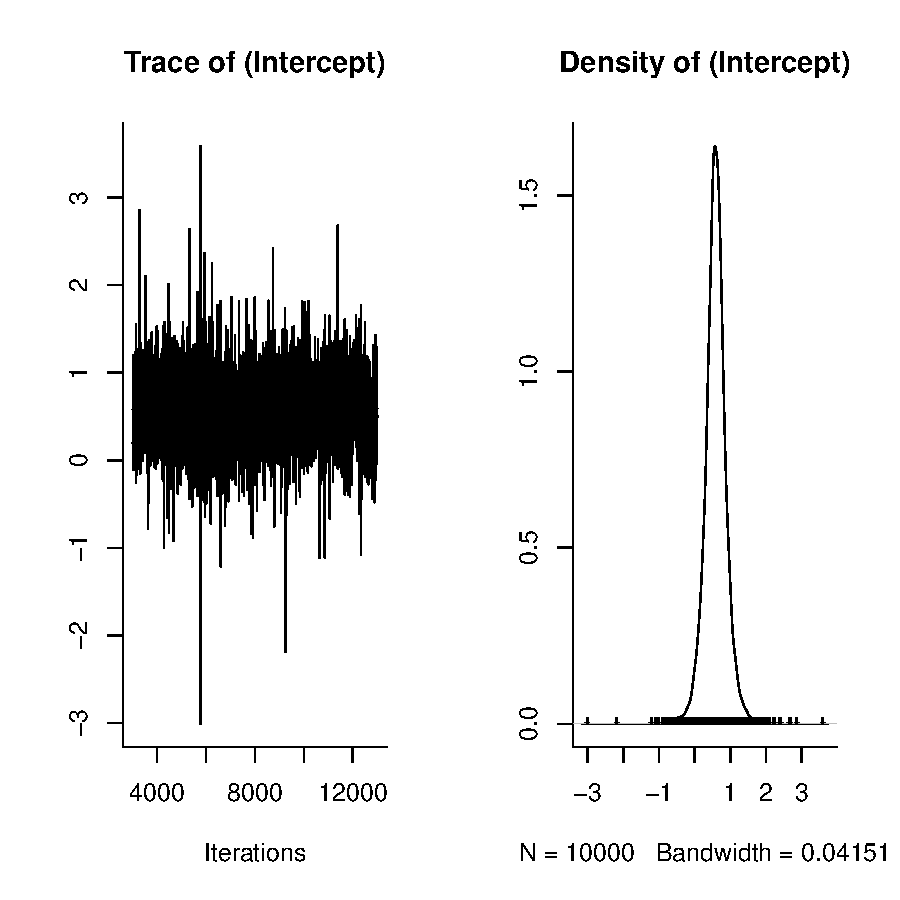
\includegraphics{Lecture1-058}
\end{center}
\caption{Summary plot of the Markov Chain for the intercept.  The left plot is a trace of the sampled posterior, and can be thought of as a time series.  The right plot is a density estimate, and can be thought of a smoothed histogram approximating the posterior.}
\label{time.series-fig}
\end{figure}

On the left of Figure \ref{time.series-fig} is a time series of the parameter as the MCMC iterates, and on the right is a posterior density estimate of the parameter (a smoothed histogram of the output). If the model has converged there should be no trend in the time series. The equivalent plot for the variance is a little hard to see on the original scale, but on the log scale the chain looks good (Figure \ref{time.series2-fig}):


\begin{Schunk}
\begin{Sinput}
> plot(log(m1a.2$VCV))
\end{Sinput}
\end{Schunk}

\begin{figure}[!h]
\begin{center}
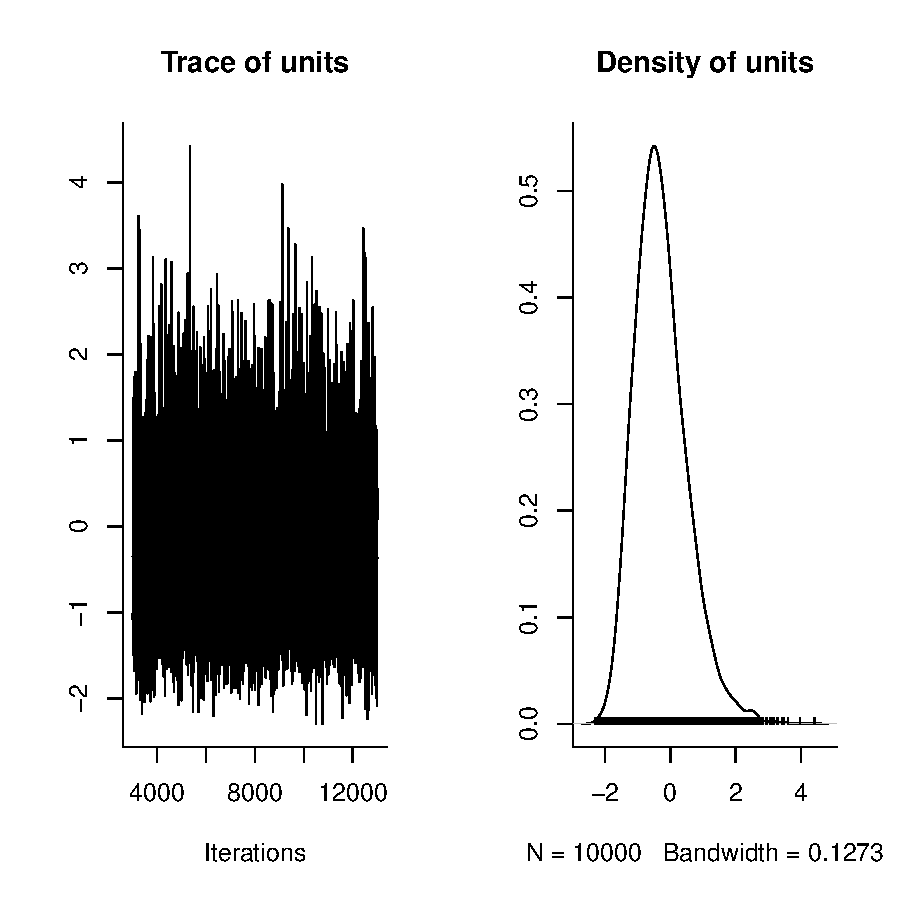
\includegraphics{Lecture1-060}
\end{center}
\caption{Summary plot of the Markov Chain for the logged variance. The logged variance was plotted rather than the variance because it was easier to visualise. The left plot is a trace of the sampled posterior, and can be thought of as a time series.  The right plot is a density estimate, and can be thought of a smoothed histogram approximating the posterior.}
\label{time.series2-fig}
\end{figure}


\section{Improper Priors}
\label{IP-sec}

When improper priors are used their are two potential problems that may be encountered. The first is that if the data do not contain enough information the posterior distribution itself may be improper, and any results obtained from \texttt{MCMCglmm} will be meaningless. In addition, with proper priors there is a zero probability of a variance component being exactly zero but this is not necessarily the case with improper priors.  This can produce numerical problems (trying to divide through by zero) and can also result in a reducible chain. A reducible chain is one which gets `stuck' at some parameter value and cannot escape. This is usually obvious from the \texttt{mcmc} plots but \texttt{MCMCglmm} will often terminate before the analysis has finished with an error message of the form:

\begin{Schunk}
\begin{Soutput}
ill-conditioned G/R structure: use proper priors ...
\end{Soutput}
\end{Schunk}  

However, improper priors do have some useful properties.
 
\subsection{Flat Improper Prior}

The simplest improper prior is one that is proportional to some constant for all possible parameter values. This is known as a flat prior and the posterior density in such cases is equal to the likelihood:

\begin{displaymath}
Pr(\mu, \sigma^{2} | {\bf y}) \propto Pr({\bf y} | \mu, \sigma^{2})
\label{fprior-eq}
\end{displaymath}

It is known that although such a prior is non-informative for the mean it is informative for the variance. We can specify a flat prior on the variance component by having \texttt{nu=0} (the value of \texttt{V} is irrelevant) and the default prior for the mean is so diffuse as to be essentially flat across the range ($-10^6, 10^6$).   

\begin{Schunk}
\begin{Sinput}
> prior.m1a.3 <- list(R = list(V = 1, nu = 0))
> m1a.3 <- MCMCglmm(y ~ 1, data = Ndata, thin = 1, 
+     prior = prior.m1a.3, verbose = FALSE)
\end{Sinput}
\end{Schunk}

We can overlay the joint posterior distribution on the likelihood surface (\ref{Psurface.flat-fig}) and see that the two things are in close agreement, up to Monte Carlo error.
 

\iftalk
\else
\fi

\begin{figure}[!h]
\begin{center}
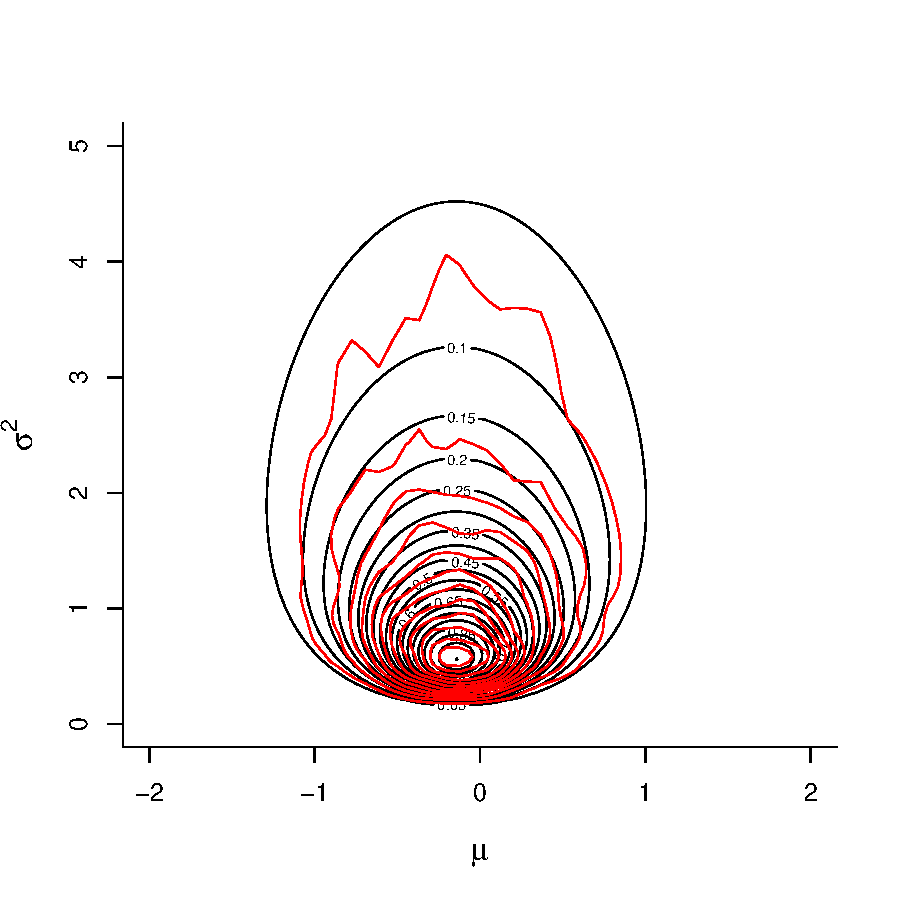
\includegraphics{Lecture1-065}
\end{center}
\caption{Likelihood surface for the likelihood $Pr({\bf y}|\mu, \sigma^{2})$ in black, and an MCMC approximation for the posterior distribution $Pr(\mu, \sigma^{2} | {\bf y})$ in red.  The likelihood has been normalised so that the maximum likelihood has a value of one, and the posterior distribution has been normalised so that the posterior mode has a value of one. Flat priors were used ($Pr(\mu)\sim N(0, 10^8)$ and  $Pr(\sigma^{2})\sim IW(\texttt{V}=0, \texttt{nu}=0)$) and so the posterior distribution is equivalent to the likelihood.}
\label{Psurface.flat-fig}
\end{figure}

\iftalk
\else
\fi
\newpage

\subsection{Non-Informative Improper Prior}

Although inverse-Wishart distributions with negative degree of belief parameters are not defined, the resulting posterior distribution can be defined if there is sufficient replication. Specifying \texttt{V=0} and \texttt{n=-1} is equivalent to a uniform prior for the standard deviation on the the interval $(0,\infty]$, and specifying \texttt{V=0} and \texttt{n=-2} is non-informative for a variance component.

\begin{Schunk}
\begin{Sinput}
> prior.m1a.4 <- list(R = list(V = 1e-16, nu = -2))
> m1a.4 <- MCMCglmm(y ~ 1, data = Ndata, thin = 1, 
+     prior = prior.m1a.4, verbose = FALSE)
\end{Sinput}
\end{Schunk}


\iftalk
\else
\fi

\begin{figure}[!h]
\begin{center}
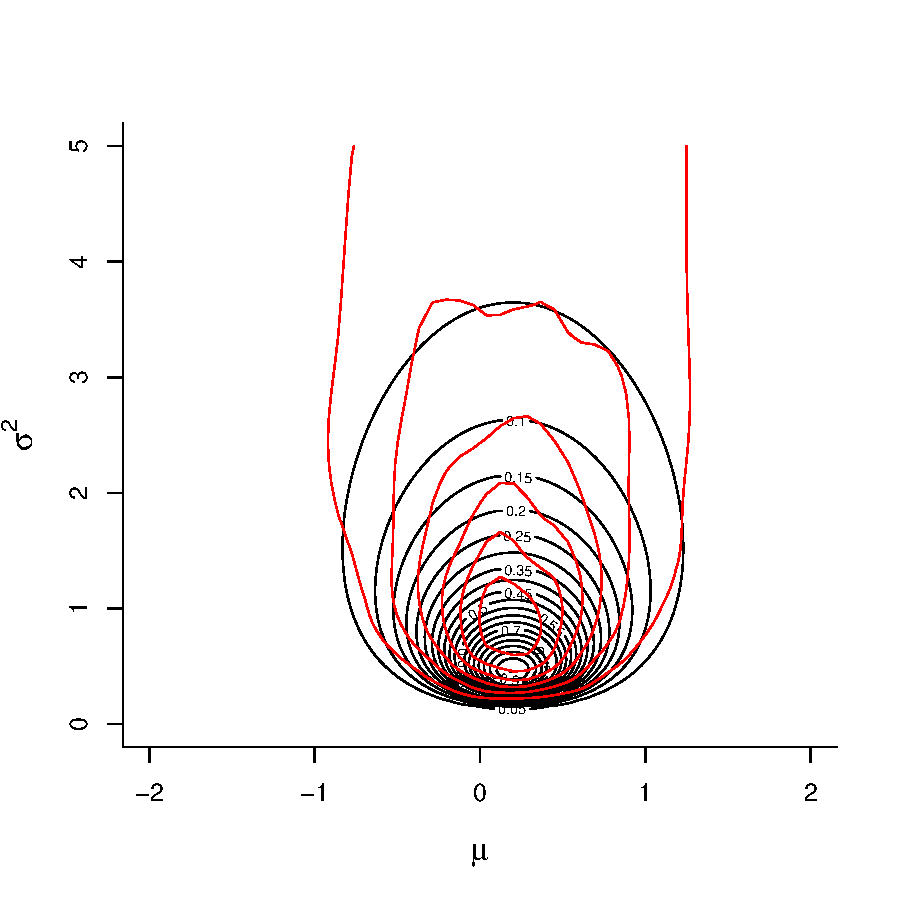
\includegraphics{Lecture1-071}
\end{center}
\caption{Likelihood surface for the likelihood $Pr({\bf y}|\mu, \sigma^{2})$ in black, and an MCMC approximation for the posterior distribution $Pr(\mu, \sigma^{2} | {\bf y})$ in red.  The likelihood has been normalised so that the maximum likelihood has a value of one, and the posterior distribution has been normalised so that the posterior mode has a value of one. A non-informative prior was used ($Pr(\mu)\sim N(0, 10^8)$ and  $Pr(\sigma^{2})\sim IW(\texttt{V}=0, \texttt{nu}=-2)$)}
\label{Psurfaceb-fig}
\end{figure}

The joint posterior mode does not coincide with either the ML or REML estimator (Figure \ref{Psurfaceb-fig}).  


but the marginal distribution of the variance component is equivalent to the REML estimator (See Figure \ref{Pmarg.NI-fig}):

\iftalk
\else
\fi

\begin{figure}[!h]
\begin{center}
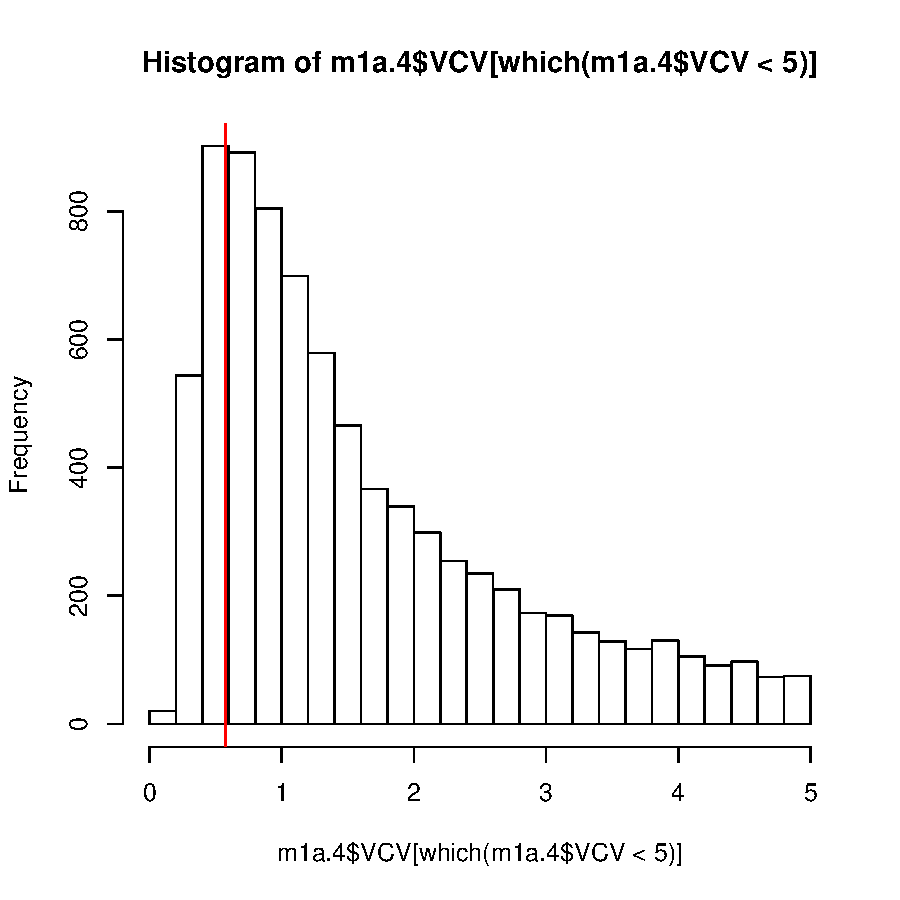
\includegraphics{Lecture1-075}
\end{center}
\caption{An MCMC approximation for the marginal posterior distribution of the variance $Pr(\sigma^{2} | {\bf y})$.  A non-informative prior specification was used ($Pr(\mu)\sim N(0, 10^8)$ and  $Pr(\sigma^{2})\sim IW(\texttt{V}=0, \texttt{nu}=-2)$) and the REML estimator of the variance (red line) coincides with the marginal posterior mode.}
\label{Pmarg.NI-fig}
\end{figure}


\ifalone
\end{document}
\else
\fi

